\documentclass{article}
\usepackage{fullpage}
\usepackage[czech]{babel}
\usepackage{amsfonts}
\usepackage{graphicx}
\usepackage{caption}
\graphicspath{{images/}}

\title{\vspace{-2cm}Mluvnice, sloh\vspace{-1.7cm}}
\date{}
\author{}

\begin{document}
\maketitle
styly: prostěsdělovací, esejistický, odborný, umělecký, řečnický, administrativní, publicistický
postupy: informační, vyprávěcí, popisný, výkladový, úvahový

\part{Odborný styl}
\begin{itemize}
  \item[a)] vědecký -- pro vědeckou veřejnost, vysoce odborný, hodně termínů
  \item[b)] učební -- pro žáky, studenty, snažíme se o něčem vzdělat někoho nevzdělaného (idk)
  \item[c)] populárně naučný -- snaží se vzdělat širší veřejnost, minimum termínů nebo jsou vysvětleny
  \item[d)] prakticky odborný -- např. návody, příručky, nějaké praktické poznatky, které můžeme využít
\end{itemize}
\begin{itemize}
  \item komposice logická, strukturovaná, bude uvedena problematika, mělo by to být přehledné, ne na přeskáčku, nějak souvisle za sebou, na konci shrnutí (resumé)
  \item anotace, abstrakt, resumé
\end{itemize}

Slohovka bude na líčení
\begin{itemize}
  \item líčení je subjektivní popis něčeho
  \item je zde velké množství obrazných pojmenování, a to především přirovnání, metafor, personifikací
  \item velmi často tím, kdo tvoří ličení je vypravěč v první osobě -- jde o vastní pocity vypravěče -- líčení v ich-formě
  \item snaha zachytit atmosféru a náš vztah k popisovanému
  \item musíme ale pořád popisovat smyslově vnímatelné okolnosti
  \item musí z toho být cítit ta emoce, to subjektivno, ten popis toho něčeho
  \item může být zabarveno i negativně, ale je to těžší
  \item cvičné líčení: oblíbené místo, hluboká noc, bouře v horách
\end{itemize}

\part{Syntax}

\section{Větné členy}
\begin{itemize}
\item základními jsou podmět a přísudek, rozvíjejícími přívlastek, předmět, příslovečné určení, doplněk
\item podmět všeobecný x vyjádřený x nevyjádřený (x vůbec není (viz \uv{Prší.}))
\item přísudek slovesný (vyjádřený slovesy, nař. vyčasovaným slovesem, vyčasovaným modálním slovesem a infinitivem, vyčasovaným fázovým slovesem a infinitivem) x jmenný se sponou (pomocné sloveso být nebo stát se a podst. nebo příd. jméno, spona může být nevyjádřena)
\item přívlastek rozvijí podst. jméno, shodný x neshodný, několikanásobný x postupně rozvitý, shodný široce rozvitý volný (Žáci, jedoucí na výlet do Drážďan, se po 2. hodině dostaví do sborovny.) x těsný (Žáci jedoucí na výlet do Drážďan se po 2. hodině dostaví do sborovny.) -- pokud přívlastek zužuje podstatné jméno (nedostaví se všichni žáci, ale právě jen ti co jedou do Drážďan) tak je těsný, bez čárek; pokud je přívlastek jen doplňková informace a obor podstatného jména se po jeho oddělení nezmění je volný a píší se okolo něj čárky
\item na předmět se ptáme jen pádovými otázkami, pokud se můžu zeptat jinak než pádovou otázkou, je to příslovečné určení, předmět bývá závislý na přísudku
\item příslovečné určení rozvíjí sloveso, příd. jm. nebo příslovce, určuje nějaké bližší okolnosti děje, přís. urč. času x místa x způsobu (prostředku (jakým prostředkem? Země byla rozpálena sluncem.), zřetele (s ohledem na co / vzhledem k čemu? Brno je bohaté na secesní památky.)) x míry (jak moc? Ranilo mě to mnoho.) x podmínky (za jaké podmínky? Při požáru utíkejte. V případě nouze mi pomůže.) x přípustky (i přes jakou okolnost? Navzdory zákazu skočil do bazénu. Přes špatné počasí jsme jeli na výlet.) x příčiny (proč ve smyslu z jakého důvodu / co je příčina? Kvůli nemoci nešel do školy. Kvůli nemoci jsme nejeli na výlet.) x účelu (proč ve smyslu za jakým účelem / co je cíl? Jí ovoce pro lepší zdraví. Šel do obchodu pro rohlíky.)
\item doplněk je zároveň závislý na podmětu i přísudku (Chlapec šel ze schodů zpívaje. -- šel zpívaje a zároveň chlapec zpívaje), jakási vlastnost jména v průběhu děje
\end{itemize}

 \begin{minipage}{0.5\paperwidth}
   \begin{itemize}
     \item větný rozbor značíme následovně:
   \end{itemize}
\end{minipage}
\hfill
\noindent\begin{minipage}{0.5\paperwidth}
    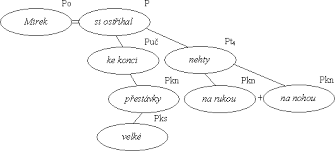
\includegraphics[width=\linewidth]{vetny_rozbor.png}
\end{minipage}
\end{document}
